\section{Comparison of MIF with other approaches}
\subsection{Overview of fusion approaches}

MIF using magnetic mirrors represents a promising approach within the diverse landscape of fusion energy research, but it exists in a broad landscape of concepts at varying levels of maturity. This report outlines some of the primary competing approaches and compares the benefits and challenges of each.

\begin{figure}[h!]
    \centering
    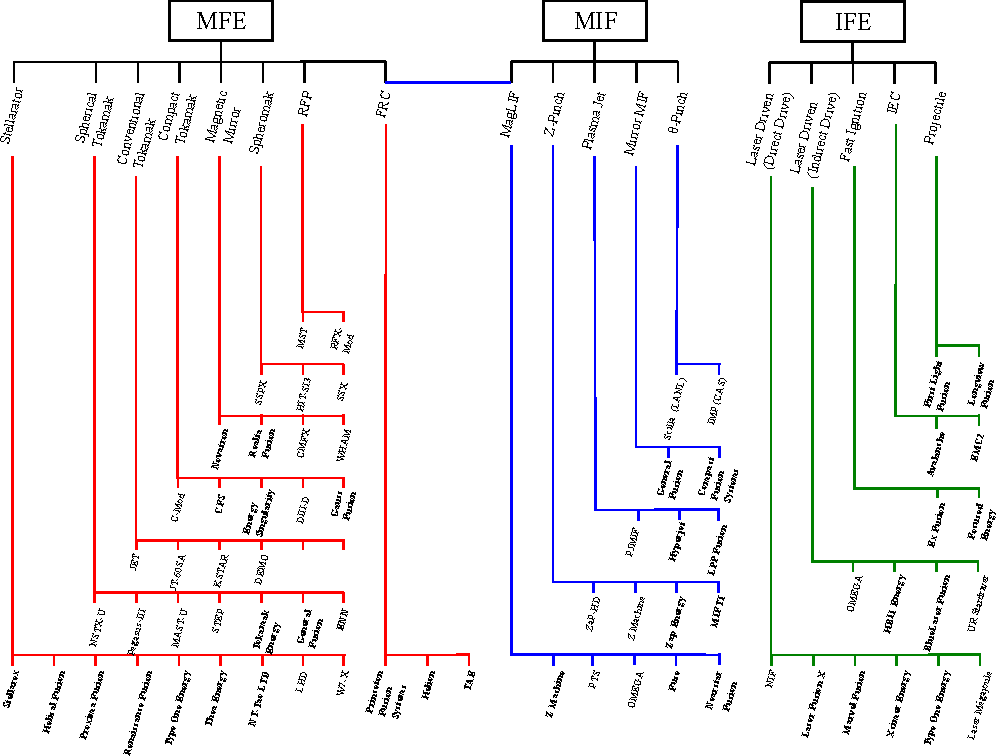
\includegraphics[width =1\linewidth]{SubreportFigures/fusion_tree_2.pdf}
    \caption{Overview of the current fusion landscape. Bold text signifies a private company.}
    \label{fig:climate_gdp}
\end{figure}

\subsubsection{MCF (Magnetic confinement fusion)}

MCF represents a dominant paradigm in fusion energy research, with Tokamaks representing the approach with by far the most funding of any fusion concept. According to the FIA 2023 report, 21 of the 42 companies surveyed are continuing MCF concepts.\\

\textbf{Tokamaks}: Tokamaks utilize a toroidal magnetic confinement system. ITER, the largest and most expensive Tokamak project to date, aims to demonstrate the feasibility of MCF as a large-scale energy source \cite{artsimovich1972tokamak}. Its design targets a Q-value (fusion power out divided by heating power in) greater than 10, with an anticipated fusion power output of 500 MW. Notably, the JET facility in the UK, which is a precursor to ITER, has provided invaluable data, especially regarding deuterium-tritium fusion reactions. Variants of the Tokamak include the compact and spherical Tokamaks which feature reduced aspect ratios. The compact design could lead to smaller, more economical fusion devices \cite{jarboe1994review}. Notably, the MAST Upgrade in the UK has been crucial in studying improved confinement modes and plasma stability. Variants on a Tokamak concept represent the most technologically mature and heavily financed fusion concept, yet have still not demonstrated net gain \cite{mirnov2018tokamak}. Owing to their significant scale (particularly for conventional aspect ratio Tokomaks), they are also generally less accessible for startups.\\

\textbf{Stellarators}: Unlike the Tokamak's symmetry around a central axis, stellarators introduce a helical twist, eliminating the need for a plasma current \cite{spitzer1958stellarator}. This design inherently reduces certain instabilities. Wendelstein 7-X in Germany, the largest stellarator in operation, aims to validate the prolonged confinement times that theoretical models predict for this configuration, with the aim of 30 minutes of continuous operation \cite{klinger2019overview}.\\

\textbf{RFPs (Reversed Field Pinches)}: RFPs use a magnetic confinement method with a magnetic field that reverses at the plasma's edge \cite{bodin1980reversed}. This design aims to offer a more stable fusion approach with less magnetic field strength compared to Tokamaks and Stellarators. Facilities such as RFX-mod in Italy have been key in exploring plasma stability and behavior in RFPs. Despite showing potential in plasma containment, RFPs still face challenges in achieving the temperatures and densities necessary for efficient fusion energy production.\\

\textbf{Spheromaks}: Spheromaks feature a self-contained smoke-ring-like magnetic configuration, aiming for a simpler and potentially more economical fusion approach \cite{jarboe1994review}. These devices, exemplified by the SSPX in the United States, are focused on studying magnetic reconnection and energy confinement. Unlike Tokamaks or Stellarators, Spheromaks do not require complex external magnetic coils, which may lead to more cost-effective solutions. However, achieving sufficient plasma pressure and maintaining stability for effective fusion remain significant challenges in spheromak research, with ongoing efforts to enhance confinement times and plasma stability.\\

\textbf{Magnetic Mirror Fusion Reactors}: Magnetic mirror reactors use magnetic fields with a "mirror" configuration to confine plasma. This setup involves creating stronger magnetic fields at both ends of the reactor, effectively trapping the plasma in between as if reflecting it between two mirrors. This concept, while simpler in design compared to Tokamaks and Stellarators, faces challenges in effectively containing the plasma for sustained periods, which are essential for achieving the conditions necessary for fusion. Magnetic mirror reactors have historically been less prominent in fusion research due to these early containment challenges and issues with plasma stability, see section \ref{mirror_lit} for a more comprehensive overview.\\


\textbf{Inertial Electrostatic Confinement (IEC)}: IEC fusion uses an electric field to confine plasma, a distinct approach from the magnetic confinement used in Tokamaks or Stellarators. In this method, a voltage applied between concentric spherical grids creates an electric field that accelerates ions toward the center, inducing fusion reactions. The design of IEC devices like Avalanche Energy's 'Marty' is notably simpler and more compact compared to other fusion methods. However, they encounter significant hurdles in achieving the necessary plasma densities and uniform conditions for effective and efficient fusion. Despite their simplicity, the feasibility of IEC devices for large-scale energy production is an area of active research and ongoing debate, and they have seen comparatively little commercial investment \cite{miley2014inertial}.\\


MCF devices, regardless of their configuration, grapple with challenges, such as the production and handling of high-energy neutrons, issues with material erosion due to plasma-wall interactions, and the complexities in achieving sustained, high-performance plasma states. With JET and ITER as notable benchmarks, the MCF approach has also been extremely costly; each extending into the 10s of billions USD.

\subsubsection{IFE (Inertial Fusion Energy)}

IFE is an alternative pathway to achieving the conditions necessary for nuclear fusion, distinguished by its rapid compression of fusion fuel.\\



\textbf{Indirect Drive IFE}: Indirect Drive IFE employs a technique where fusion fuel pellets are placed inside a hohlraum, which is then irradiated by lasers. The National Ignition Facility (NIF), a leading research center for Indirect Drive, has recently achieved a major milestone in demonstrating net energy gain, where the fusion energy output exceeded the energy input from the lasers \cite{miller2004national}. This achievement is significant, as it provides a proof-of-concept for the viability of Indirect Drive IFE as a potential energy source. However, challenges specific to this approach include refining laser targeting and energy delivery to improve efficiency, managing the high costs associated with large-scale laser systems, and developing materials that can withstand the extreme conditions of fusion reactions. These hurdles must be overcome to transition from experimental demonstrations to practical, scalable fusion power plants. Despite these challenges, Indirect Drive IFE remains a promising area in fusion research, with ongoing efforts aimed at resolving these technical issues.\\

\textbf{Direct Drive Inertial IFE}: Direct Drive IFE, exemplified by research at facilities like the OMEGA Laser Facility, directly targets fusion fuel pellets with high-energy beams, such as lasers or particle beams \cite{soures1996direct}. Similar to Indirect Drive, it faces challenges like the development of advanced laser systems and durable materials to withstand intense fusion conditions. However, the primary challenge of Direct Drive is achieving the high degree of precision and symmetry in beam delivery necessary for uniform pellet compression and stable fusion reactions \cite{bodner1998direct}. This precision is critical for the success and efficiency of the method. Direct Drive continues to be a significant area of research, striving to address these technical hurdles to transform the concept into a practical energy solution.\\




\textbf{Fast Ignition Fusion IFE}: Fast Ignition is a technique that divides the fusion process into compression and ignition phases. A high-energy driver first compresses the fusion fuel pellet, followed by a short, intense pulse that rapidly heats a portion of the fuel to ignite fusion. This approach aims to enhance efficiency by potentially reducing the total energy required for fusion. Coordinating these stages precisely, which involves sophisticated technology and a comprehensive understanding of plasma physics, is a key challenge. Notable experiments in Fast Ignition have been conducted at facilities like the Laboratory for Laser Energetics in the United States, highlighting its potential. However, Fast Ignition still faces significant technical hurdles in its development towards a feasible energy solution.\\



\textbf{Projectile Inertial Fusion Energy (IFE)}: Projectile IFE is a fusion approach where high-speed projectiles are fired at a target containing fusion fuel, aiming to induce fusion through intense compression and heating. This method diverges from traditional magnetic or electrostatic confinement techniques, instead relying on kinetic impact to achieve the necessary conditions for fusion. The concept involves precisely synchronizing the projectile impact to maximize compression and temperature of the fuel pellet, triggering fusion reactions \cite{jha2020incomplete}. While the idea of using kinetic energy for fusion is innovative, it presents significant technical challenges, particularly in projectile acceleration, targeting accuracy, and managing the resulting high-energy impacts. Current notable efforts are underway at first light fusion in the UK.








%\begin{figure}[h!]
%\centering
%\includegraphics[scale=0.4]{fusion_tree.pdf}
%\caption{Taxonomy of fusion approaches.} 
%\label{fig:taxonomy} 
%\end{figure}




\subsubsection{MIF (Magnetic Inertial Fusion)}

MIF techniques, including FRC and other configurations, bridge the principles of magnetic and inertial confinement, and operate in the intermediate particle density regime %PUT FIG HERE.

\begin{figure}[h!]
    \centering
    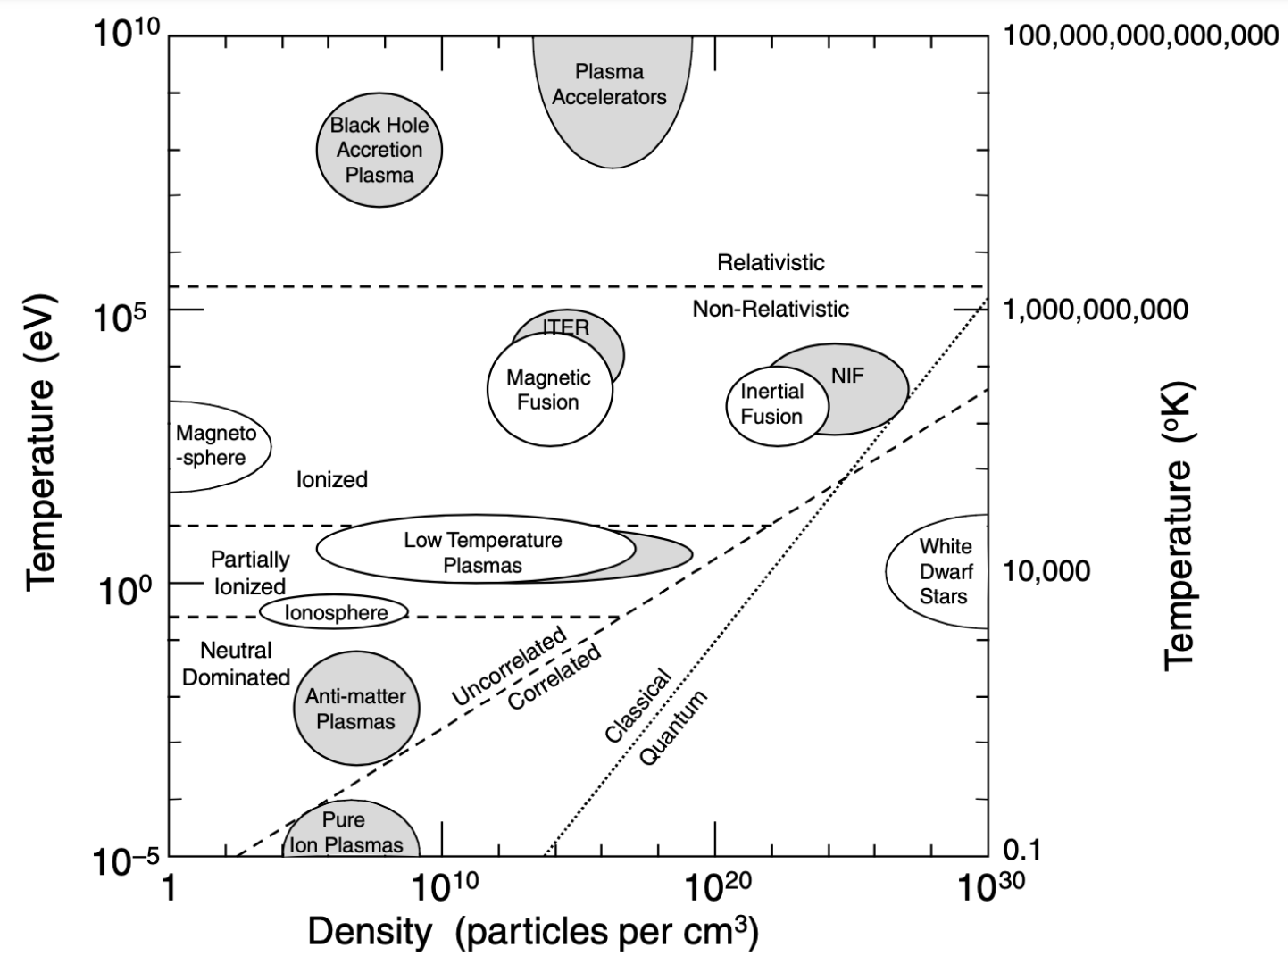
\includegraphics[width =0.65\linewidth]{SubreportFigures/density_regimes.pdf}
    \caption{Illustrative representation of density regimes of various MCF, IFE and MIF experiments and other phenomena for context. From \cite{xiao2021stochastic}. }
    \label{fig:climate_gdp}
\end{figure}

\textbf{Field-Reversed Configuration (FRC)}: FRC is a toroidal plasma configuration devoid of a central magnetic field, which differentiates it from Tokamaks and Stellarators. TAE Technologies’ Norman reactor is a noteworthy experiment in this domain, having recently achieved lifetimes that make it viable for power production scenarios. While the compact nature of FRCs is appealing, issues such as sustaining the configuration without instabilities and achieving the needed confinement times for fusion conditions persist.\\

\textbf{MagLIF}: This method, studied extensively at Sandia, seeks to synchronize lasers, magnetic fields, and pulsed power to achieve fusion conditions. While the integration of these techniques offers a promising route, the challenge lies in mastering the intricacies of their coordination.

\textbf{Plasma Jet MIF}: Plasma Jet fusion employs high-velocity plasma jets to compress and heat fusion fuel pellets, a technique distinct from the laser or particle beam methods used in Direct and Indirect Drive. The key challenge lies in generating and controlling plasma jets with the necessary speed, density, and stability for effective fusion. This approach requires advanced technologies for plasma generation and acceleration, as well as precision in jet targeting and timing. Despite its potential for efficient energy delivery to the fusion fuel, Plasma Jet MIF is still in the early stages of research, with significant technical hurdles to overcome in transitioning from experimental research to a viable fusion energy source.

\textbf{Z Pinch}: Z-pinch devices utilize a cylindrical magnetic confinement approach for fusion energy compressing plasma along the z-axis using a strong axial magnetic field, generated by a high-current electrical discharge \cite{zhang2019sustained}. The MAGPIE project, a leading Z Pinch experiment, aims to understand and control plasma instabilities inherent to this approach \cite{shumlak2020z}. It focuses on achieving high plasma temperatures and densities, essential for initiating fusion reactions. A key characteristic of Z Pinch is its potential for pulsed power fusion, where brief but intense fusion reactions are triggered during the compression phase.

One notable variant is the Sheared-Flow Stabilized Z Pinch, which stabilizes the plasma by imposing a velocity shear along the axial direction \cite{shumlak2001evidence}. This variant shows promise in mitigating destructive plasma instabilities, a major challenge in the Z Pinch approach. The ZaP and ZaP-HD experiments at the University of Washington have been instrumental in demonstrating the effectiveness of sheared flow in stabilizing Z Pinch plasmas.

Despite their potential for simpler and more compact designs, Z Pinch devices, including their variants, have yet to demonstrate a net gain in fusion energy output \cite{velikovich2015z}. However, their relative accessibility and lower cost make them attractive for smaller-scale research and startup ventures in the fusion energy sector.



\subsection{Comparisons}


\begin{table}[h!]
    \centering
    \begin{tabular}{cccccc}
        \hline
        \makecell{Concept} & \makecell{Technological Maturity \\ (TRL)} & \makecell{Economic Viability \\ (assuming physics)} & \makecell{Environmental Impact} & \makecell{Safety (LSA)} \\
        \hline
        IFE - DT & 3 & Good & Medium & 2\\
        IFE - D-$^3$He & 2 & Excellent & Low & 1\\
        IFE - pB11 & 2 & Excellent & Low & 1\\
        MFE - DT & 3 & Good & Medium & 2\\
        MFE - D-$^3$He & 2 & Excellent & Low & 1 \\
        MIF - DT & 2 & Good & Low & 2\\
        MIF D-$^3$He & 1 & Excellent & Medium & 1\\
        \hline
    \end{tabular}
    \caption{Comparative overview of the status of the various main approaches to fusion. *assuming $^3$He can be sourced. }
    \label{tab:my_label}
\end{table}
